\documentclass[]{book}
\usepackage{lmodern}
\usepackage{amssymb,amsmath}
\usepackage{ifxetex,ifluatex}
\usepackage{fixltx2e} % provides \textsubscript
\ifnum 0\ifxetex 1\fi\ifluatex 1\fi=0 % if pdftex
  \usepackage[T1]{fontenc}
  \usepackage[utf8]{inputenc}
\else % if luatex or xelatex
  \ifxetex
    \usepackage{mathspec}
  \else
    \usepackage{fontspec}
  \fi
  \defaultfontfeatures{Ligatures=TeX,Scale=MatchLowercase}
\fi
% use upquote if available, for straight quotes in verbatim environments
\IfFileExists{upquote.sty}{\usepackage{upquote}}{}
% use microtype if available
\IfFileExists{microtype.sty}{%
\usepackage{microtype}
\UseMicrotypeSet[protrusion]{basicmath} % disable protrusion for tt fonts
}{}
\usepackage{hyperref}
\hypersetup{unicode=true,
            pdftitle={Research Methods},
            pdfborder={0 0 0},
            breaklinks=true}
\urlstyle{same}  % don't use monospace font for urls
\usepackage{color}
\usepackage{fancyvrb}
\newcommand{\VerbBar}{|}
\newcommand{\VERB}{\Verb[commandchars=\\\{\}]}
\DefineVerbatimEnvironment{Highlighting}{Verbatim}{commandchars=\\\{\}}
% Add ',fontsize=\small' for more characters per line
\usepackage{framed}
\definecolor{shadecolor}{RGB}{248,248,248}
\newenvironment{Shaded}{\begin{snugshade}}{\end{snugshade}}
\newcommand{\AlertTok}[1]{\textcolor[rgb]{0.94,0.16,0.16}{#1}}
\newcommand{\AnnotationTok}[1]{\textcolor[rgb]{0.56,0.35,0.01}{\textbf{\textit{#1}}}}
\newcommand{\AttributeTok}[1]{\textcolor[rgb]{0.77,0.63,0.00}{#1}}
\newcommand{\BaseNTok}[1]{\textcolor[rgb]{0.00,0.00,0.81}{#1}}
\newcommand{\BuiltInTok}[1]{#1}
\newcommand{\CharTok}[1]{\textcolor[rgb]{0.31,0.60,0.02}{#1}}
\newcommand{\CommentTok}[1]{\textcolor[rgb]{0.56,0.35,0.01}{\textit{#1}}}
\newcommand{\CommentVarTok}[1]{\textcolor[rgb]{0.56,0.35,0.01}{\textbf{\textit{#1}}}}
\newcommand{\ConstantTok}[1]{\textcolor[rgb]{0.00,0.00,0.00}{#1}}
\newcommand{\ControlFlowTok}[1]{\textcolor[rgb]{0.13,0.29,0.53}{\textbf{#1}}}
\newcommand{\DataTypeTok}[1]{\textcolor[rgb]{0.13,0.29,0.53}{#1}}
\newcommand{\DecValTok}[1]{\textcolor[rgb]{0.00,0.00,0.81}{#1}}
\newcommand{\DocumentationTok}[1]{\textcolor[rgb]{0.56,0.35,0.01}{\textbf{\textit{#1}}}}
\newcommand{\ErrorTok}[1]{\textcolor[rgb]{0.64,0.00,0.00}{\textbf{#1}}}
\newcommand{\ExtensionTok}[1]{#1}
\newcommand{\FloatTok}[1]{\textcolor[rgb]{0.00,0.00,0.81}{#1}}
\newcommand{\FunctionTok}[1]{\textcolor[rgb]{0.00,0.00,0.00}{#1}}
\newcommand{\ImportTok}[1]{#1}
\newcommand{\InformationTok}[1]{\textcolor[rgb]{0.56,0.35,0.01}{\textbf{\textit{#1}}}}
\newcommand{\KeywordTok}[1]{\textcolor[rgb]{0.13,0.29,0.53}{\textbf{#1}}}
\newcommand{\NormalTok}[1]{#1}
\newcommand{\OperatorTok}[1]{\textcolor[rgb]{0.81,0.36,0.00}{\textbf{#1}}}
\newcommand{\OtherTok}[1]{\textcolor[rgb]{0.56,0.35,0.01}{#1}}
\newcommand{\PreprocessorTok}[1]{\textcolor[rgb]{0.56,0.35,0.01}{\textit{#1}}}
\newcommand{\RegionMarkerTok}[1]{#1}
\newcommand{\SpecialCharTok}[1]{\textcolor[rgb]{0.00,0.00,0.00}{#1}}
\newcommand{\SpecialStringTok}[1]{\textcolor[rgb]{0.31,0.60,0.02}{#1}}
\newcommand{\StringTok}[1]{\textcolor[rgb]{0.31,0.60,0.02}{#1}}
\newcommand{\VariableTok}[1]{\textcolor[rgb]{0.00,0.00,0.00}{#1}}
\newcommand{\VerbatimStringTok}[1]{\textcolor[rgb]{0.31,0.60,0.02}{#1}}
\newcommand{\WarningTok}[1]{\textcolor[rgb]{0.56,0.35,0.01}{\textbf{\textit{#1}}}}
\usepackage{longtable,booktabs}
\usepackage{graphicx,grffile}
\makeatletter
\def\maxwidth{\ifdim\Gin@nat@width>\linewidth\linewidth\else\Gin@nat@width\fi}
\def\maxheight{\ifdim\Gin@nat@height>\textheight\textheight\else\Gin@nat@height\fi}
\makeatother
% Scale images if necessary, so that they will not overflow the page
% margins by default, and it is still possible to overwrite the defaults
% using explicit options in \includegraphics[width, height, ...]{}
\setkeys{Gin}{width=\maxwidth,height=\maxheight,keepaspectratio}
\IfFileExists{parskip.sty}{%
\usepackage{parskip}
}{% else
\setlength{\parindent}{0pt}
\setlength{\parskip}{6pt plus 2pt minus 1pt}
}
\setlength{\emergencystretch}{3em}  % prevent overfull lines
\providecommand{\tightlist}{%
  \setlength{\itemsep}{0pt}\setlength{\parskip}{0pt}}
\setcounter{secnumdepth}{5}
% Redefines (sub)paragraphs to behave more like sections
\ifx\paragraph\undefined\else
\let\oldparagraph\paragraph
\renewcommand{\paragraph}[1]{\oldparagraph{#1}\mbox{}}
\fi
\ifx\subparagraph\undefined\else
\let\oldsubparagraph\subparagraph
\renewcommand{\subparagraph}[1]{\oldsubparagraph{#1}\mbox{}}
\fi

%%% Use protect on footnotes to avoid problems with footnotes in titles
\let\rmarkdownfootnote\footnote%
\def\footnote{\protect\rmarkdownfootnote}

%%% Change title format to be more compact
\usepackage{titling}

% Create subtitle command for use in maketitle
\providecommand{\subtitle}[1]{
  \posttitle{
    \begin{center}\large#1\end{center}
    }
}

\setlength{\droptitle}{-2em}

  \title{Research Methods}
    \pretitle{\vspace{\droptitle}\centering\huge}
  \posttitle{\par}
    \author{}
    \preauthor{}\postauthor{}
      \predate{\centering\large\emph}
  \postdate{\par}
    \date{2019-11-25}

\usepackage{booktabs}
\usepackage{amsthm}
\makeatletter
\def\thm@space@setup{%
  \thm@preskip=8pt plus 2pt minus 4pt
  \thm@postskip=\thm@preskip
}
\makeatother

\AtBeginDocument{\let\maketitle\relax} % supress header


\usepackage{fancyhdr}

\pagestyle{fancy}
% \fancyhead[CO,CE]{ZHAW LSFM}
\fancyfoot[CO,CE]{\textsc{zhaw lsfm}}
\fancyfoot[LE,RO]{\thepage}
\fancyfoot[RE,LO]{Modul \textit{ResearchMethods}}

\begin{document}
\maketitle

\newgeometry{tmargin=1.5cm,lmargin=2.5cm,rmargin=2.5cm,bmargin=0.5cm} %verbose

\begin{titlepage}
\begin{center}
  
{\small 
ZURICH UNIVERSITY OF APPLIED SCIENCES
\linebreak SCHOOL OF LIFE SCIENCES AND FACILITY MANAGEMENT
\linebreak INSTITUTE OF NATURAL RESOURCE SCIENCES
}

\end{center}
\vspace{1.5cm}
\begin{center}

{\Large Übungsunterlagen und Demoscript zum Modul \emph{Research Methods}}

\end{center}
 \vspace{1cm}

% \begin{figure}[htbp]
%   \centering
%   \includegraphics[width=1\textwidth]{Images/Reh-flucht-compilation3_small.png}
%   \label{titelbild} 
% \end{figure}

\begin{center}
\textbf{Herbstsemester 2019}

%\textbf{Patrick Laube und Nils Ratnaweera}

\end{center} 

\vspace{1.0cm}


\newpage
\thispagestyle{empty}
\begin{minipage}{15cm}
\begin{flushleft}




\vspace{18cm}
{\large Impressum:}

\vspace{0.5cm}

% \textbf{Citation:} 
Laube, P. et al. (2019): Übungsunterlagen für das Modul Research Methods im Master of Science in Umwelt und Natürliche Ressourcen. IUNR, Zürcher Hochschule der Angewandten Wissenschaften (ZHAW), W{\"a}denswil.

\end{flushleft}
\end{minipage}

\end{titlepage}
\restoregeometry

{
\setcounter{tocdepth}{1}
\tableofcontents
}
\hypertarget{einleitung}{%
\chapter{Einleitung}\label{einleitung}}

Das Modul „Research Methods`` vermittelt vertiefte Methodenkompetenzen für praxisorientiertes und angewandtes wissenschaftliches Arbeiten im Fachbereich „Umwelt und Natürliche Ressourcen`` auf MSc-Niveau. Die Studierenden erarbeiten sich vertiefte Methodenkompetenzen für die analytische Betrachtung der Zusammenhänge im Gesamtsystem „Umwelt und Natürliche Ressourcen``. Die Studierenden erlernen die methodischen Kompetenzen, auf denen die nachfolgenden Module im MSc Programm UNR aufbauen. Das Modul vermittelt einerseits allgemeine, fächerübergreifende methodische Kompetenzen (z.B. Wissenschaftstheorie, computer-gestützte Datenverar-beitung und Statistik).

Auf dieser Plattform (RStudio Connect) werden die Unterlagen für die R-Übungsteile bereitgestellt. Es werden sukzessive sowohl Demo-Files, Aufgabenstellungen und Lösungen veröffentlicht.

\hypertarget{raumanalyse-1-25.11.2019}{%
\chapter{Raumanalyse 1 (25.11.2019)}\label{raumanalyse-1-25.11.2019}}

Die erste Übung zur Raumanalyse illustriert das einfache Laden und Anzeigen von Geodaten im Vektor- und Raster-Datenformat. Zusätzlich veranschaulicht die Übung den Umgang mit Koordinatensystemen sowie die Vektor-Raster-Konvertierung. Einfach erste Analysen umfassen den Spatial Join (Annotieren von Punkten mit Attributen von die Punkte einbettenden Vektordaten) sowie Puffer-Operationen. Zum Abschluss thematisiert die Übung die Aggregationsabhängigkeit räumlicher Daten durch die Illustration des Modifiable Areal Unit Problem (MAUP). Inhaltlich orientiert sich die Übung an Bodeneigenschaften für den Untersuchungsraum Schweiz.

\hypertarget{ubung-spatial-join-puffer-und-maup}{%
\section{Übung: Spatial Join, Puffer und MAUP}\label{ubung-spatial-join-puffer-und-maup}}

\hypertarget{themantische-einbettung}{%
\subsection{Themantische Einbettung}\label{themantische-einbettung}}

Mit dieser Übung wirst Du Schritt fürfür Schritt an einfache Methoden der Raumanalyse herangeführt. Dies umfasst das Laden und Plotten von Vektor- und Rasterdaten sowie den wichtigen Umgang mit Koordinatensystemen. Darauf folgen einige Übungen zur räumlichen Anreicherung von Punktdaten unter Verwendung des Konzepts des ``Spatial Join''. Dazu arbeiten wir mit einem Datensatz aus Punktstichproben zur Wasserverfügbarkeit in Schweizer Böden. Es soll untersucht werden, ob ein Zusammenhang besteht zwischen der an den Punkten gemessenen Wasserverfügbarkeit und dem Join-Layer Bodeneignung/Skelettanteil. Im zweiten Teil der Übung wirst Du die Messwerte zur Wasserverfügbarkeit auf unterschiedlichen räumlichen Skalen aggregieren (Kantone, Bezirke und Gemeinden) und prüfen, ob ggf. das Modifiable Areal Unit Problem auftritt.

\hypertarget{vorbereitung}{%
\subsection{Vorbereitung}\label{vorbereitung}}

Es gibt bereits eine Vielzahl von Packages um in R mit räumlichen Daten zu arbeiten, die ihrerseits wiederum auf weiteren Packages basieren (Stichwort \texttt{dependencies}).

\begin{itemize}
\tightlist
\item
  Für \emph{Vektordaten} dominierte lange das Package \texttt{sp}, welches nun aber schrittweise durch \texttt{sf} abgelöst wird. Wir werden wenn immer möglich mit \texttt{sf} arbeiten und nur in Ausnahmefällen auf andere Packages zurück greifen.
\item
  Für \emph{Rasterdaten} exisitert das Package \texttt{raster}
\end{itemize}

Für die Integration von Vektor und Rasterdaten existiert das Package \texttt{starts}: \textbf{S}patio\textbf{t}emporal \textbf{A}rrays for \textbf{R}aster and \textbf{V}ector Datacubes. Diese Tools sind teilweise sehr gut dem Tidyverse-Workflow (\texttt{group\_by}, \texttt{mutate}, \texttt{summarise}, \texttt{\%\textgreater{}\%}) integriert. Lade zu beginn die folgenden notwenigen Packages (installiere die fehlenden Packages mit \texttt{install.package("packagename")}).

\begin{Shaded}
\begin{Highlighting}[]
\KeywordTok{library}\NormalTok{(sf)}
\KeywordTok{library}\NormalTok{(tidyverse)}
\KeywordTok{library}\NormalTok{(stars)}
\KeywordTok{library}\NormalTok{(raster)}
\end{Highlighting}
\end{Shaded}

\hypertarget{aufgabe-1-daten-runterladen-und-importieren}{%
\subsection{Aufgabe 1: Daten runterladen und importieren}\label{aufgabe-1-daten-runterladen-und-importieren}}

Lade zunächst die Datensätze unter folgenden Links herunter und importiere sie mit dem Befehl \texttt{read\_sf()} in R:

\begin{itemize}
\tightlist
\item
  \href{21_RaumAn1/data/skelettgehalt_proben.gpkg}{bodeneignung\_skelett.gpkg}: Datensatz des Bundesamt für Landwirtschaft, modifiziert (\href{https://www.blw.admin.ch/blw/de/home/politik/datenmanagement/geografisches-informationssystem-gis/download-geodaten.html}{weitere Informationen})
\item
  \href{21_RaumAn1/data/kantone.gpkg}{kantone.gpkg}: Ein Datensatz der Swisstopo, modifiziert (\href{https://shop.swisstopo.admin.ch/de/products/landscape/boundaries3D}{weitere Informationen})
\item
  \href{21_RaumAn1/data/bezirke.gpkg}{bezirke.gpkg}: Ein Datensatz der Swisstopo, modifiziert (\href{https://shop.swisstopo.admin.ch/de/products/landscape/boundaries3D}{weitere Informationen})
\item
  \href{21_RaumAn1/data/wasserverfuegbarkeit_boden.gpkg}{wasserverfuegbarkeit\_boden.gpkg}: Ein Datensatz der WSL, modifiziert (\href{https://www.wsl.ch/de/ueber-die-wsl/programme-und-initiativen/abgeschlossene-programme-und-grossprojekte/wuk.html}{weiteren Informationen})
\end{itemize}

Es handelt sich um Geodatensätze im Format Geopackage (``*.gpkg''), eine alternatives Datenformat zum bekannteren Format ``Shapefiles''. Lade nun die Datensätze wie folgt ein:

\begin{Shaded}
\begin{Highlighting}[]

\CommentTok{# Pfad muss natürlich angepasst werden}
\NormalTok{wasser <-}\StringTok{ }\KeywordTok{read_sf}\NormalTok{(}\StringTok{"21_RaumAn1/data/wasserverfuegbarkeit_boden.gpkg"}\NormalTok{)}
\NormalTok{kantone <-}\StringTok{ }\KeywordTok{read_sf}\NormalTok{(}\StringTok{"21_RaumAn1/data/kantone.gpkg"}\NormalTok{)}
\NormalTok{bezirke <-}\StringTok{ }\KeywordTok{read_sf}\NormalTok{(}\StringTok{"21_RaumAn1/data/bezirke.gpkg"}\NormalTok{) }
\NormalTok{gemeinden <-}\StringTok{ }\KeywordTok{read_sf}\NormalTok{(}\StringTok{"21_RaumAn1/data/gemeinden.gpkg"}\NormalTok{)}
\NormalTok{skelettgehalt <-}\StringTok{ }\KeywordTok{read_sf}\NormalTok{(}\StringTok{"21_RaumAn1/data/bodeneignung_skelett.gpkg"}\NormalTok{)}
\end{Highlighting}
\end{Shaded}

Schau Dir die importierten Datensätze an, nutzt dafür \texttt{View()}, \texttt{str()}, \texttt{class()}. Studiere ausserdem die weiteren Informationen zu den Datensätzen.

\hypertarget{aufgabe-2-daten-visualisieren}{%
\subsection{Aufgabe 2: Daten Visualisieren}\label{aufgabe-2-daten-visualisieren}}

Wir hatten anfangs erwähnt, dass Geodaten mit \texttt{sf} und \texttt{raster} sich teilweise sehr schön in die bekannten Tidyverse workflows integrieren lassen. Das merkt man schnell, wenn man die Daten visualisieren möchte. In InfoVis 1 \& 2 haben wir intensiv mit \texttt{ggplot2} gearbeitet und dort die Layers \texttt{geom\_point()} und \texttt{geom\_line()} kennen gelernt. Zusätzlich beinhaltet \texttt{ggplot} die Möglichkeit, mit \texttt{geom\_sf()} Vektordaten direkt und sehr einfach zu plotten. Führe die angegebenen R-Befehle aus und studiere die entstehenden Plots. Welche Unterschiede findest Du? Wie erklärst Du diese Unterschiede?

\begin{Shaded}
\begin{Highlighting}[]
\KeywordTok{ggplot}\NormalTok{(bezirke) }\OperatorTok{+}\StringTok{ }
\StringTok{  }\KeywordTok{geom_sf}\NormalTok{()}
\end{Highlighting}
\end{Shaded}

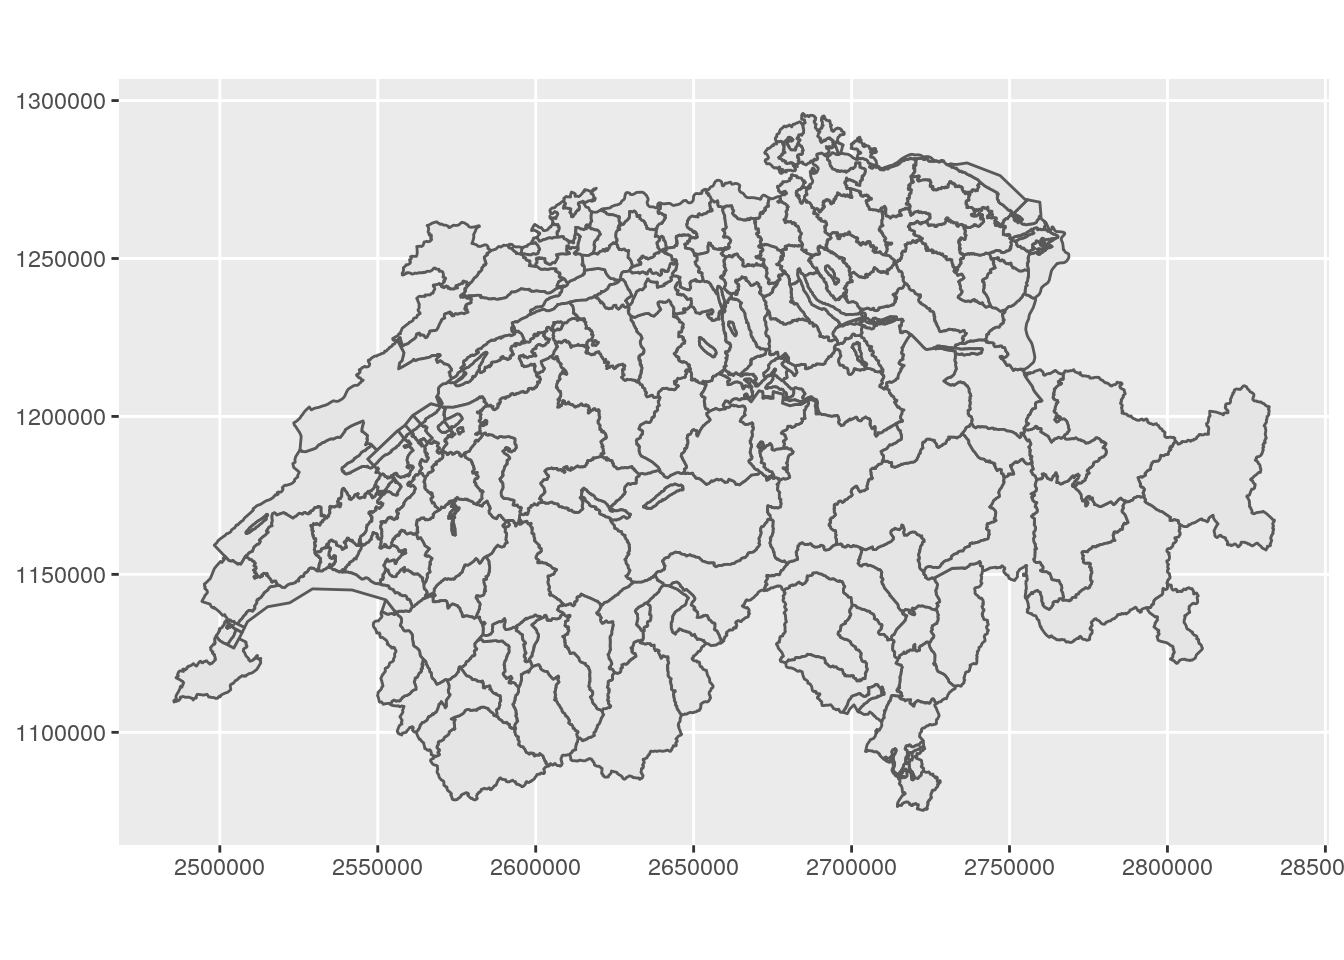
\includegraphics{_main_files/figure-latex/unnamed-chunk-8-1.pdf}

\begin{Shaded}
\begin{Highlighting}[]
\KeywordTok{ggplot}\NormalTok{(wasser) }\OperatorTok{+}\StringTok{ }
\StringTok{  }\KeywordTok{geom_sf}\NormalTok{()}
\end{Highlighting}
\end{Shaded}

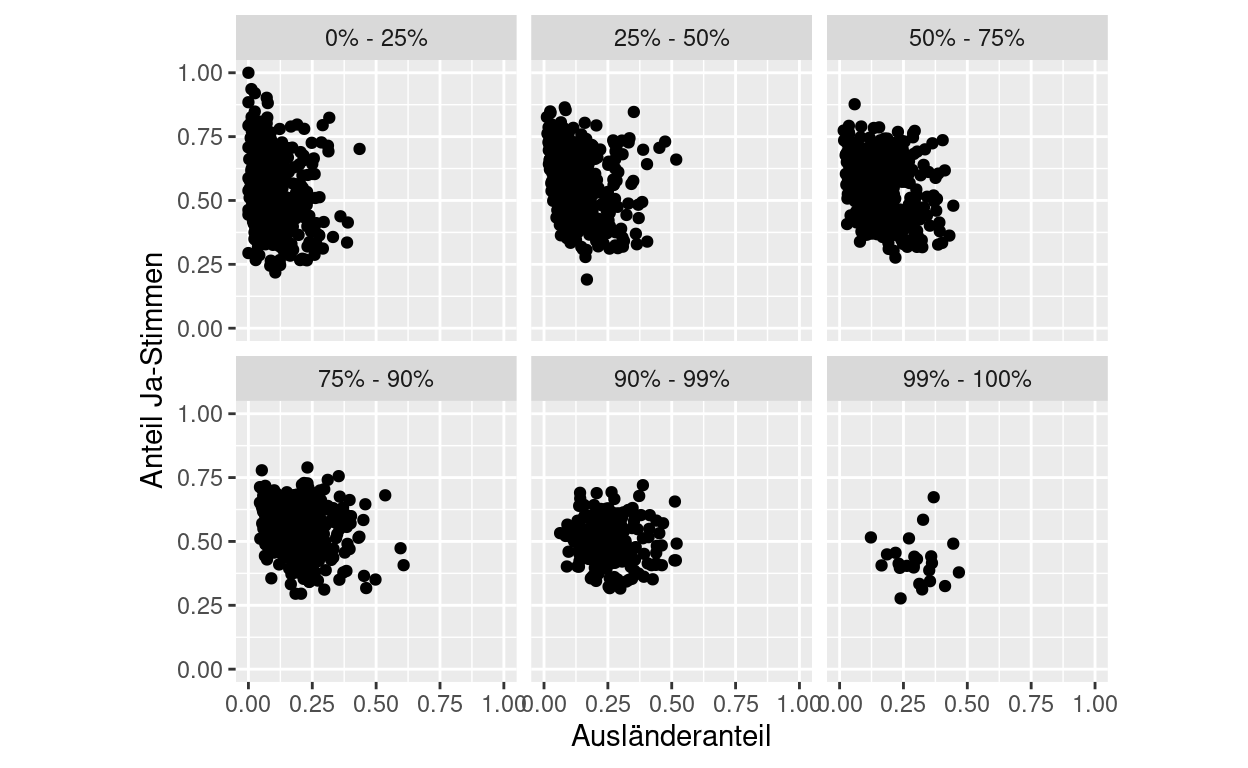
\includegraphics{_main_files/figure-latex/unnamed-chunk-9-1.pdf}

\hypertarget{aufgabe-3-koordinatensysteme-zuweisen}{%
\subsection{\texorpdfstring{Aufgabe 3 Koordinatensysteme \emph{zuweisen}}{Aufgabe 3 Koordinatensysteme zuweisen}}\label{aufgabe-3-koordinatensysteme-zuweisen}}

In den obigen beiden sehr einfachen Kartogrammen fallen verschiedene Dinge auf:

\begin{itemize}
\tightlist
\item
  die X/Y Achsen weisen zwei ganz unterschiedlichen Zahlenbereiche auf (vergleiche die Achsenbeschriftungen), und
\item
  der Umriss der Schweiz scheint im zweiten Plot ``gestaucht'' zu sein.
\end{itemize}

Dies hat natürlich damit zu tun, dass die beiden Datensätze in unterschiedlichen Koordinatensystemen erfasst wurden. Koordinatensysteme werden mit CRS (\textbf{C}oordinate \textbf{R}eference \textbf{S}ystem) abgekürzt. Mit \texttt{st\_crs()} könnnen die zugewiesenen Koordinatensysteme abgefragt werden.

\begin{Shaded}
\begin{Highlighting}[]
\KeywordTok{st_crs}\NormalTok{(wasser)}
\CommentTok{## Coordinate Reference System: NA}
\KeywordTok{st_crs}\NormalTok{(bezirke)}
\CommentTok{## Coordinate Reference System: NA}
\end{Highlighting}
\end{Shaded}

Leider sind in unserem Fall keine Koordinatensysteme zugewiesen. Mit etwas Erfahrung kann man das Koordinatensystem aber erraten, so viele kommen nämlich gar nicht in Frage. Am häufigsten trifft man hierzulande eines der drei folgenden Koordinatensysteme an:

\begin{itemize}
\tightlist
\item
  \href{https://epsg.io/21781}{CH1903 LV03}: das alte Koordinatensystem der Schweiz
\item
  \href{https://epsg.io/2056}{CH1903+ LV95}: das neue Koordinatensystem der Schweiz
\item
  \href{https://epsg.io/4326}{WGS84}: ein häufig genutztes weltumspannendes geodätisches Koordinatensystem, sprich die Koordinaten werden in Länge und Breite angegeben (Lat/Lon).
\end{itemize}

Nun gilt es, anhand der Koordinaten die in der Spalte \texttt{geometry} ersichtlich sind das korrekte Koordinatensystem festzustellen. Wenn man sich auf \href{https://epsg.io/map\#srs=4326\&x=8.407288\&y=46.773731\&z=9\&layer=streets}{epsg.io/map} die Schweiz anschaut, kann man die Koordinaten in verschiedenen Koordinatensystem betrachten.

\textbf{Bedienungshinweise}:

\begin{figure}
\centering

\includegraphics{koordinatenpaar.jpg}
\caption{Koordinanten (des Fadenkreuzes) werden im ausgewählten Koordinatensystem dargestellt}
\end{figure}

\begin{figure}
\centering
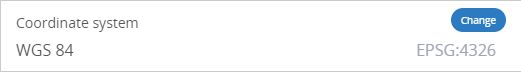
\includegraphics{koordinatensystem.jpg}
\caption{Das Koordinatensystem, in welchem die Koordinaten dargestellt werden sollen, kann mit ``Change'' angepasst werden}
\end{figure}

\begin{figure}
\centering

\includegraphics{reproject.jpg}
\caption{Für Enthusiasten: Schau Dir die Schweiz in verschiedenen Koordinatensystemen an, in dem Du auf ``Reproject Map'' klickst}
\end{figure}

Wenn man diese Koordinaten mit den Koordinaten unserer Datensätze vergleicht, dann ist schnell klar, dass es sich beim Datensatz \texttt{wasser} um das Koordinatensystem WGS84 handelt und bei \texttt{bezirke} das Koordinatensystem CH1903+ LV95. Diese Koordinatensyteme weisen wir nun mit \texttt{st\_set\_crs()} und dem entsprechenden \emph{EPSG}-Code (siehe die jeweiligen Links) zu.

\begin{Shaded}
\begin{Highlighting}[]
\NormalTok{wasser <-}\StringTok{ }\KeywordTok{st_set_crs}\NormalTok{(wasser, }\DecValTok{4326}\NormalTok{)}
\NormalTok{bezirke <-}\StringTok{ }\KeywordTok{st_set_crs}\NormalTok{(bezirke, }\DecValTok{2056}\NormalTok{)}

\CommentTok{# zuweisen mit st_set_crs(), abfragen mit st_crs()}
\KeywordTok{st_crs}\NormalTok{(wasser)}
\CommentTok{## Coordinate Reference System:}
\CommentTok{##   EPSG: 4326 }
\CommentTok{##   proj4string: "+proj=longlat +datum=WGS84 +no_defs"}
\end{Highlighting}
\end{Shaded}

Weise auch für die anderen Datensätze (\texttt{kantone}, \texttt{gemeinden}, \texttt{skelettgehalt}) das \emph{korrekte} Koordinatensytem zu.

Jetzt wo das CRS der Datensätze bekannt ist, können diese in einem gemeinsamen Plot visualisiert werden, \texttt{ggplot} kümmert sich darum die unterschiedlichen Koordinatensysteme zu vereinheitlichen. Probier das aus, indem du \texttt{kantone} und \texttt{wasser} in einem \texttt{ggplot} kombinierst.

Die Achsen werden dann immer in WGS84 beschriftet. Wenn das stört, kann man \texttt{coord\_sf(datum\ =\ 2056)} in einem weiteren Layer spezifizieren. Oder aber man blendet die Achsenbeschriftung mit \texttt{theme\_void()} komplett aus. Versuche beide Varianten.

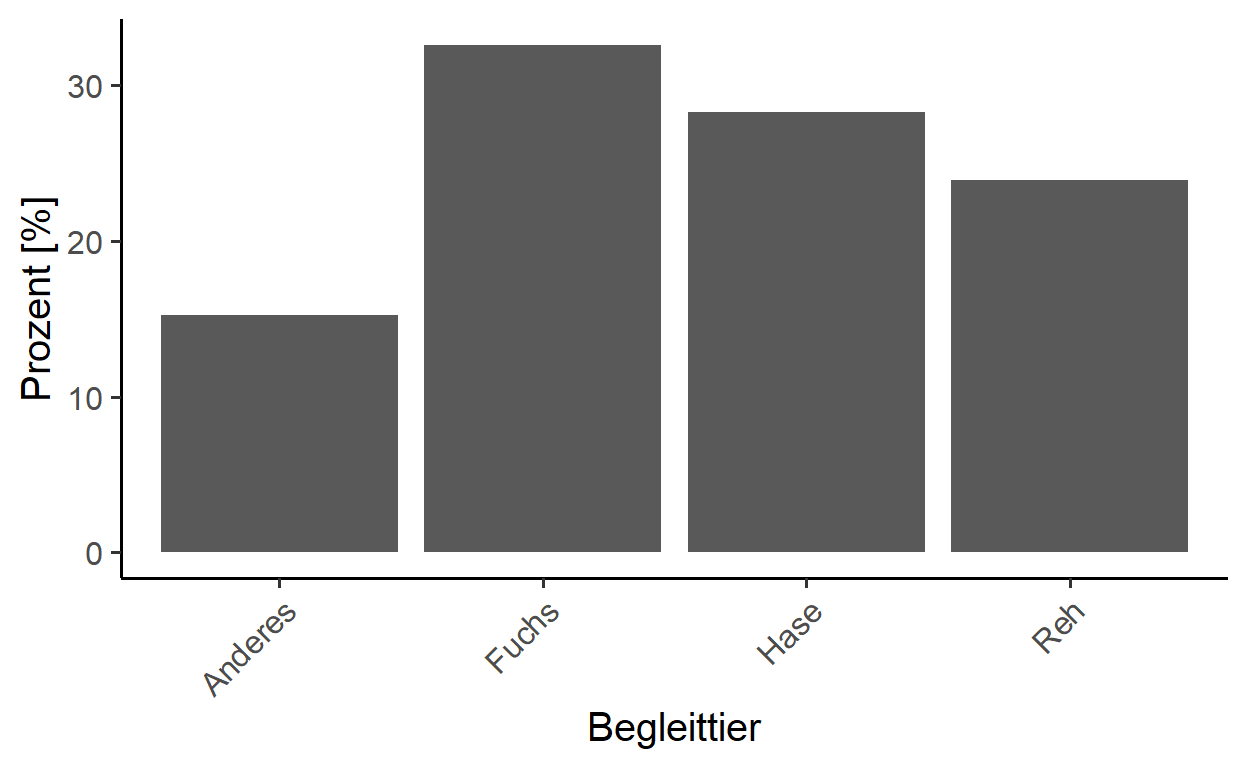
\includegraphics{_main_files/figure-latex/unnamed-chunk-13-1.pdf}

\hypertarget{aufgabe-4-koordinatensyteme-transformieren}{%
\subsection{\texorpdfstring{Aufgabe 4: Koordinatensyteme \emph{transformieren}}{Aufgabe 4: Koordinatensyteme transformieren}}\label{aufgabe-4-koordinatensyteme-transformieren}}

In der vorherigen Übung haben wir das bestehende Koordinatensystem \emph{zugewiesen}. Dabei haben wir die bestehenden Koordinaten (in der Spalte \texttt{geom}) \emph{nicht} manipuliert. Ganz anders ist eine \emph{Transformation} der Daten von einem Koordinatensystem in das andere. Bei einer Transformation werden die Koordinaten in das neue Koordinatensystem umgerechnet und somit manipuliert. Aus praktischen Gründen wollen
wir all unsere Daten ins neue Schweizer Koordinatensystem CH1903+ LV95 transfomieren. Transformiere den Datensatz \texttt{wasser} mit \texttt{st\_transform()}in CH1903+ LV95, nutze dafür den korrekten EPSG-Code.

Vor der Transformation (betrachte die Spalte \texttt{geom} sowie die Attribute \texttt{epsg\ (SRID)} und \texttt{proj4string}):

\begin{Shaded}
\begin{Highlighting}[]
\NormalTok{wasser}
\CommentTok{## Simple feature collection with 993 features and 1 field}
\CommentTok{## geometry type:  POINT}
\CommentTok{## dimension:      XY}
\CommentTok{## bbox:           xmin: 6.006132 ymin: 45.84509 xmax: 10.46693 ymax: 47.76851}
\CommentTok{## epsg (SRID):    4326}
\CommentTok{## proj4string:    +proj=longlat +datum=WGS84 +no_defs}
\CommentTok{## # A tibble: 993 x 2}
\CommentTok{##    wasserverfuegbarkeit                geom}
\CommentTok{##                   <dbl>         <POINT [°]>}
\CommentTok{##  1                 -167 (8.997155 45.84509)}
\CommentTok{##  2                    0 (7.072459 45.91802)}
\CommentTok{##  3                    0 (7.153695 45.90636)}
\CommentTok{##  4                    0 (7.251192 45.91059)}
\CommentTok{##  5                    0 (7.380257 45.92894)}
\CommentTok{##  6                    0 (7.423909 45.92544)}
\CommentTok{##  7                    0 (9.013727 45.91338)}
\CommentTok{##  8                  -91 (9.051913 45.89967)}
\CommentTok{##  9                    0  (7.069596 45.9689)}
\CommentTok{## 10                 -102  (7.175481 45.9782)}
\CommentTok{## # ... with 983 more rows}
\end{Highlighting}
\end{Shaded}

Nach der Transformation (betrachte die Spalte \texttt{geom}):

\begin{Shaded}
\begin{Highlighting}[]
\NormalTok{wasser}
\CommentTok{## Simple feature collection with 993 features and 1 field}
\CommentTok{## geometry type:  POINT}
\CommentTok{## dimension:      XY}
\CommentTok{## bbox:           xmin: 2489453 ymin: 1078252 xmax: 2830887 ymax: 1291537}
\CommentTok{## epsg (SRID):    2056}
\CommentTok{## proj4string:    +proj=somerc +lat_0=46.95240555555556 +lon_0=7.439583333333333 +k_0=1 +x_0=2600000 +y_0=1200000 +ellps=bessel +towgs84=674.374,15.056,405.346,0,0,0,0 +units=m +no_defs}
\CommentTok{## # A tibble: 993 x 2}
\CommentTok{##    wasserverfuegbarkeit              geom}
\CommentTok{##                   <dbl>       <POINT [m]>}
\CommentTok{##  1                 -167 (2721079 1078252)}
\CommentTok{##  2                    0 (2571587 1085224)}
\CommentTok{##  3                    0 (2577885 1083902)}
\CommentTok{##  4                    0 (2585453 1084350)}
\CommentTok{##  5                    0 (2595470 1086373)}
\CommentTok{##  6                    0 (2598856 1085983)}
\CommentTok{##  7                    0 (2722214 1085868)}
\CommentTok{##  8                  -91 (2725207 1084404)}
\CommentTok{##  9                    0 (2571392 1090881)}
\CommentTok{## 10                 -102 (2579603 1091882)}
\CommentTok{## # ... with 983 more rows}
\end{Highlighting}
\end{Shaded}

\hypertarget{aufgabe-5}{%
\subsection{Aufgabe 5:}\label{aufgabe-5}}

Wir wollen nun wissen, ob die Wasserverfügbarkeit im Boden mit dem Skelettgehalt zusammen hängt. Dazu nutzen wir die GIS-Technik \emph{Spatial Join}, die in der Vorlesung beschrieben wurde. In \texttt{sf} können wir Spatial Joins mit der Funktion \texttt{st\_join} durchführen, dabei gibt es nur \texttt{left} sowie \texttt{inner}-Joins (vgl. PrePro 1 \& 2). So müssen die Punkte ``Links'', also an erste Stelle aufgeführt werden, da wir ja Attribute \emph{an} die Punkte anheften wollen.

\begin{verbatim}
## Simple feature collection with 993 features and 2 fields
## geometry type:  POINT
## dimension:      XY
## bbox:           xmin: 2489453 ymin: 1078252 xmax: 2830887 ymax: 1291537
## epsg (SRID):    2056
## proj4string:    +proj=somerc +lat_0=46.95240555555556 +lon_0=7.439583333333333 +k_0=1 +x_0=2600000 +y_0=1200000 +ellps=bessel +towgs84=674.374,15.056,405.346,0,0,0,0 +units=m +no_defs
## # A tibble: 993 x 3
##    wasserverfuegbarkeit              geom SKELETT
##                   <dbl>       <POINT [m]>   <dbl>
##  1                 -167 (2721079 1078252)       3
##  2                    0 (2571587 1085224)      NA
##  3                    0 (2577885 1083902)      NA
##  4                    0 (2585453 1084350)      NA
##  5                    0 (2595470 1086373)      NA
##  6                    0 (2598856 1085983)      NA
##  7                    0 (2722214 1085868)       4
##  8                  -91 (2725207 1084404)       4
##  9                    0 (2571392 1090881)      NA
## 10                 -102 (2579603 1091882)       4
## # ... with 983 more rows
\end{verbatim}

Führe den obigen Spatial Join aus und erstelle anschliessend einen Boxplot pro Skelett-Kategorie. Für \texttt{ggplot} boxplots ist es sinnvoll, den Skelettgehalt vorgängig von \texttt{numeric} in \texttt{factor} zu konvertieren (falls Du nicht mehr weisst weshalb, schau nochmals nach in PrePro und InfoVis).

Nun haben wir das Ziel der Aufgabe erreicht und die Messpunkte durch räumliche Zusatzinformation aufgewertet. Wir werden das Resultat an dieser Stelle aber nicht weiter interpretieren, dass wäre Teil einer Bodenkunde Vorlesung.

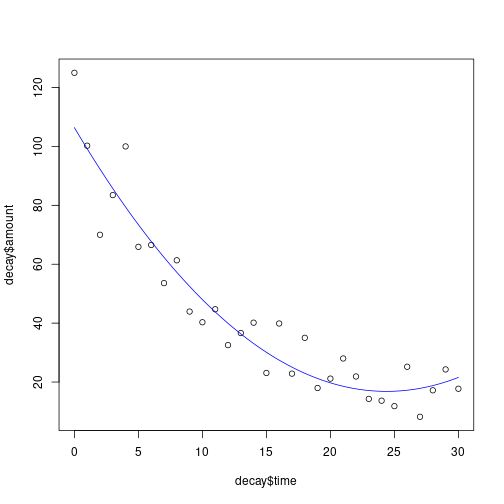
\includegraphics{_main_files/figure-latex/unnamed-chunk-18-1.pdf}

\hypertarget{aufgabe-6-spatial-join-mit-flachen}{%
\subsection{Aufgabe 6: Spatial Join mit Flächen}\label{aufgabe-6-spatial-join-mit-flachen}}

In der letzten Aufgabe haben wir für jede Probe aus \texttt{wasser} den Skelettgehalt des darunterliegenden Polygons ermittelt. Für Proben, die gerade an der Grenze zu einem Polygon mit einem anderen Skelettgehalt liegen ist dieser Wert aber nicht sehr aussagekräftig.

So könnte es zum Beispiel wichtiger sein zu wissen, was \emph{der dominierende Skelettgehalt innerhalb eines 2 km Radius} um die Probe ist. In den kommenden Teilaufgaben lösen wir diese Herausforderung.

\hypertarget{teilaufgabe-a-punkte-mit-puffer-versehen}{%
\subsubsection{Teilaufgabe A: Punkte mit Puffer versehen}\label{teilaufgabe-a-punkte-mit-puffer-versehen}}

Dafür müssen wir die Punkte mit einem Puffer versehen. Dies erreichen wir mit \texttt{st\_buffer()}. Erstelle einen Datensatz \texttt{wasser\_2km}, in dem jeder Punkt mit 2'000 m gepuffert wurde. Visualisiere dann diesen Datensatz. Beachte, dass es sich nun nicht mehr um Punkte, sondern um Flächen handelt (\texttt{POLYGON}).

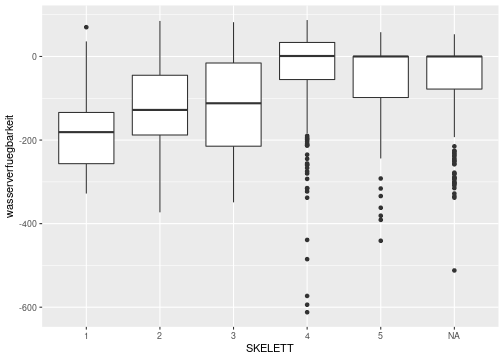
\includegraphics{_main_files/figure-latex/unnamed-chunk-20-1.pdf}

\hypertarget{teilaufgabe-b-vektordatensatz-in-raster-konvertieren}{%
\subsubsection{Teilaufgabe B: Vektordatensatz in Raster konvertieren}\label{teilaufgabe-b-vektordatensatz-in-raster-konvertieren}}

Um Flächen miteinander zu verrechnen (``Was ist der dominierende Skelettgehalt im Umkreis von 2km?'') ist es einfacher, wenn der Skelettgehalt-Datensatz im Raster-Datenformat daher kommt. Dazu wandeln wir den Vektordatensatz \texttt{skelettgehalt} mit einer Vektor-nach-Raster-Konvertierung in den Rasterdatensatz \texttt{skelett\_raster}. Hierzu brauchen wir die Funktion \texttt{fasterize()} (\textbf{f}ast \textbf{rasterize}) aus der gleichnamigen Library. Installiere diese Library (wenn nötig) und importiere sie in die aktuelle Session mit \texttt{library(fasterize)}.

In einem ersten Schritt müssen wir eine Raster-Vorlage erstellen, welche dazu dient, die räumliche Ausdehnung und die Auflösung (Zellengrösse) des resultierenden Datensatzes festzulegen.

\begin{Shaded}
\begin{Highlighting}[]
\KeywordTok{library}\NormalTok{(fasterize)}

\NormalTok{raster_template <-}\StringTok{ }\KeywordTok{raster}\NormalTok{(}\KeywordTok{extent}\NormalTok{(skelettgehalt), }\DataTypeTok{resolution =} \DecValTok{1000}\NormalTok{)}
\end{Highlighting}
\end{Shaded}

Danach wird mit \texttt{fasterize} der Polygon-Datensatz in ein Raster konvertiert. Mit \texttt{field\ =} kann festgelegt werden, aus welcher Spalte die Werte des Output Datensatzes entnommen werden sollten. GIS-Experten werden sich erinnern, dass im Gegensatz zu Flächen in einem Vektordatensatz, welche viele verschiedene Attributen haben können, ein Raster nur noch ein Attribut (hier \texttt{SKELETT}).

\begin{Shaded}
\begin{Highlighting}[]
\NormalTok{skelett_raster <-}\StringTok{ }\KeywordTok{fasterize}\NormalTok{(skelettgehalt,raster_template,}\DataTypeTok{field =} \StringTok{"SKELETT"}\NormalTok{)}

\KeywordTok{ggplot}\NormalTok{() }\OperatorTok{+}\StringTok{ }
\StringTok{  }\KeywordTok{geom_stars}\NormalTok{(}\DataTypeTok{data =} \KeywordTok{st_as_stars}\NormalTok{(skelett_raster)) }\OperatorTok{+}
\StringTok{  }\KeywordTok{coord_equal}\NormalTok{()}
\end{Highlighting}
\end{Shaded}

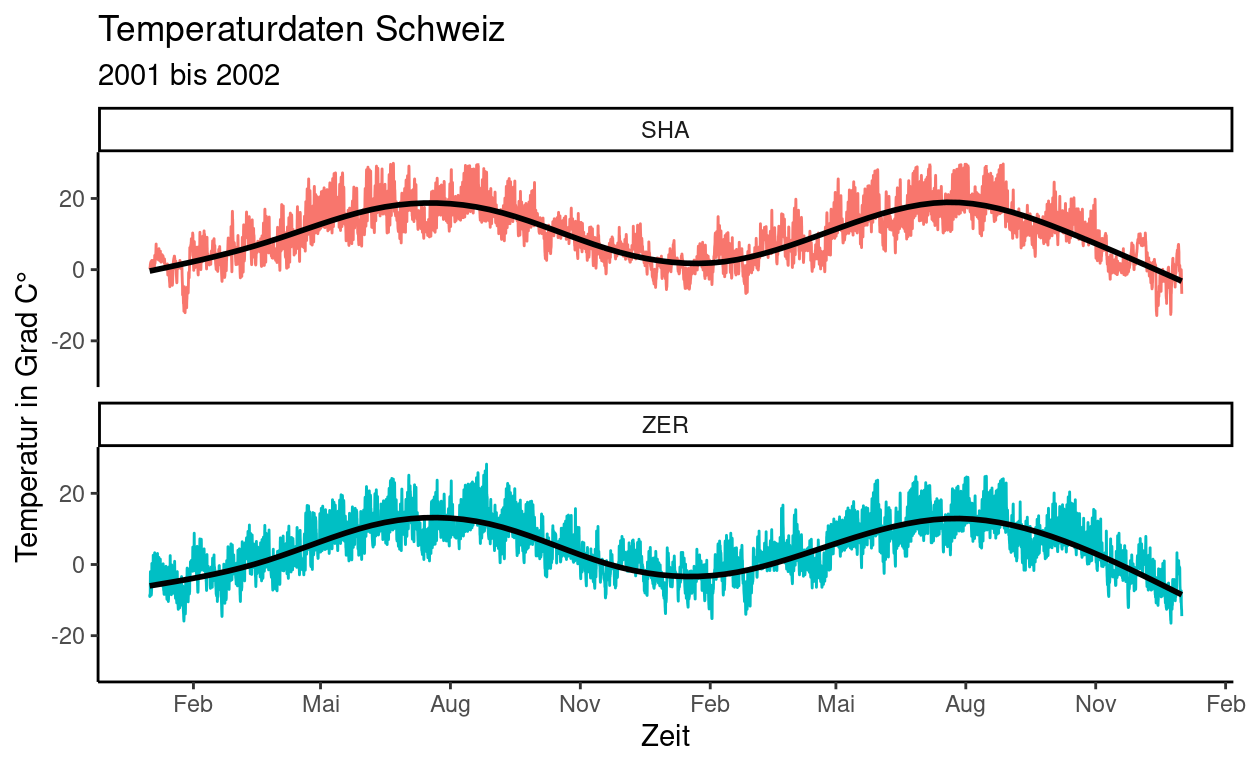
\includegraphics{_main_files/figure-latex/unnamed-chunk-22-1.pdf}

\hypertarget{teilaufgabe-c-rasterwerte-extrahieren}{%
\subsubsection{Teilaufgabe C: Rasterwerte extrahieren}\label{teilaufgabe-c-rasterwerte-extrahieren}}

Mit \texttt{raster::extract()} könnnen nun die Rasterwerte aus dem Rasterdatensatz extrahiert werden. In \texttt{fun\ =} kann festgelegt werden, ob und mit welcher Funktion die vielen Rasterzellen pro Polygon aggregiert werden sollen. Wir möchten nur den häufigsten Wert zurück erhalten, sprich den \href{https://de.wikipedia.org/wiki/Modus_(Statistik)}{Modus} dafür gibt es in \texttt{R} leider keine eingebaute Funktion, weshalb wir unsere eigene basteln müssen:

\begin{Shaded}
\begin{Highlighting}[]
\NormalTok{mode <-}\StringTok{ }\ControlFlowTok{function}\NormalTok{(x,}\DataTypeTok{na.rm =} \OtherTok{FALSE}\NormalTok{) \{}
\NormalTok{  ux <-}\StringTok{ }\KeywordTok{unique}\NormalTok{(x)}
\NormalTok{  ux[}\KeywordTok{which.max}\NormalTok{(}\KeywordTok{tabulate}\NormalTok{(}\KeywordTok{match}\NormalTok{(x, ux)))]}
\NormalTok{\}}
\end{Highlighting}
\end{Shaded}

Nun können wir mit \texttt{raster::extract()} den Modus in jedem Puffer berechnen.

\begin{Shaded}
\begin{Highlighting}[]
\NormalTok{wasser_skelett}\OperatorTok{$}\NormalTok{skelett_mode <-}\StringTok{ }\KeywordTok{extract}\NormalTok{(skelett_raster,wasser_2km,}\DataTypeTok{fun =}\NormalTok{ mode)[,}\DecValTok{1}\NormalTok{]}
\end{Highlighting}
\end{Shaded}

Jetzt könnnen wir prüfen, wie oft die beiden Join-Varianten übereinstimmen. Erstelle dazu einen Facet-Plot, indem für jede Skelett-Kategorie die Modus-Kategorie (sprich die häufigste Kategorie) im den Punkt umgebenden Puffer darstellt.

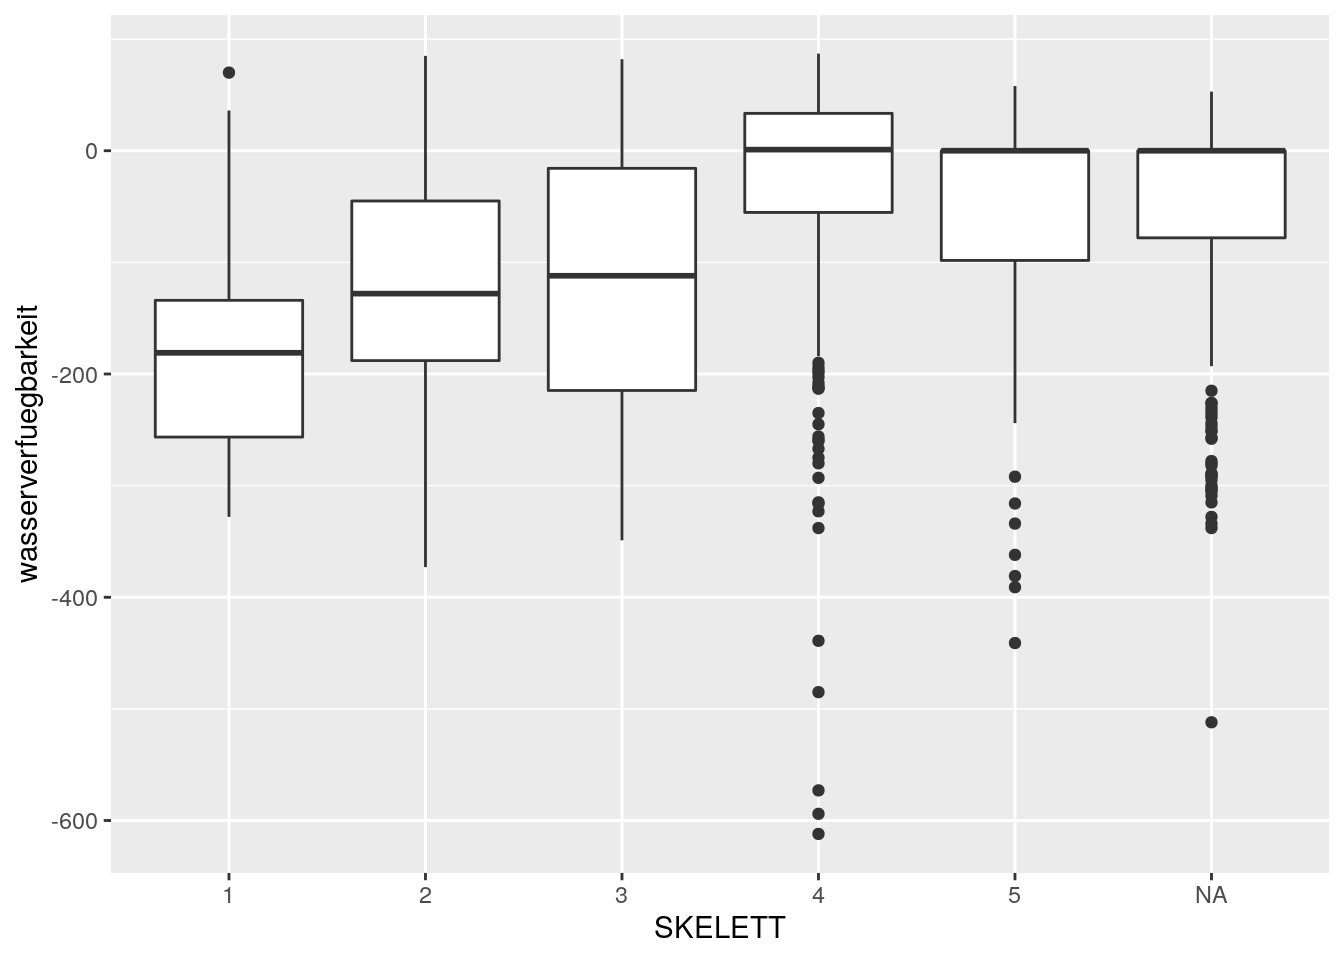
\includegraphics{_main_files/figure-latex/unnamed-chunk-25-1.pdf}

\hypertarget{aufgabe-7-spatial-join-mit-kantone-bezirke-gemeinden}{%
\subsection{Aufgabe 7: Spatial Join mit Kantone, Bezirke, Gemeinden}\label{aufgabe-7-spatial-join-mit-kantone-bezirke-gemeinden}}

Zum Abschluss der Übung wenden wir uns nun noch der Aggregationsabhängigkeit von Geodaten zu. Dazu wollen wir die Daten zur Wasserverfügbarkeit auf verschiedenen Massstäben aggregieren. Als Aggregationseinheiten verwenden wir die politische Gliederung der Schweit - Kantone, Bezirke und Gemeinden. Die Frage stellt sich, ob die Daten ev. das MAUP illustrieren.

Hier könnten wir wir nochmals \texttt{st\_join()} verwenden, aber da wir diesmal Polygone im Fokus haben (Bezirke, Kantone) und mehrere Punkte in einem Polygon vorkommen können, ist dieser Weg etwas umständlich. Wir nutzen deshalb die Funktion \texttt{aggregate()}, und spezifizieren \texttt{x\ =\ wasser}, \texttt{by\ =\ kantone} und \texttt{FUN\ =\ mean}.

Hinweis: Das Beschriften der Kantone ist fakultativ und nicht \emph{ganz} trivial.

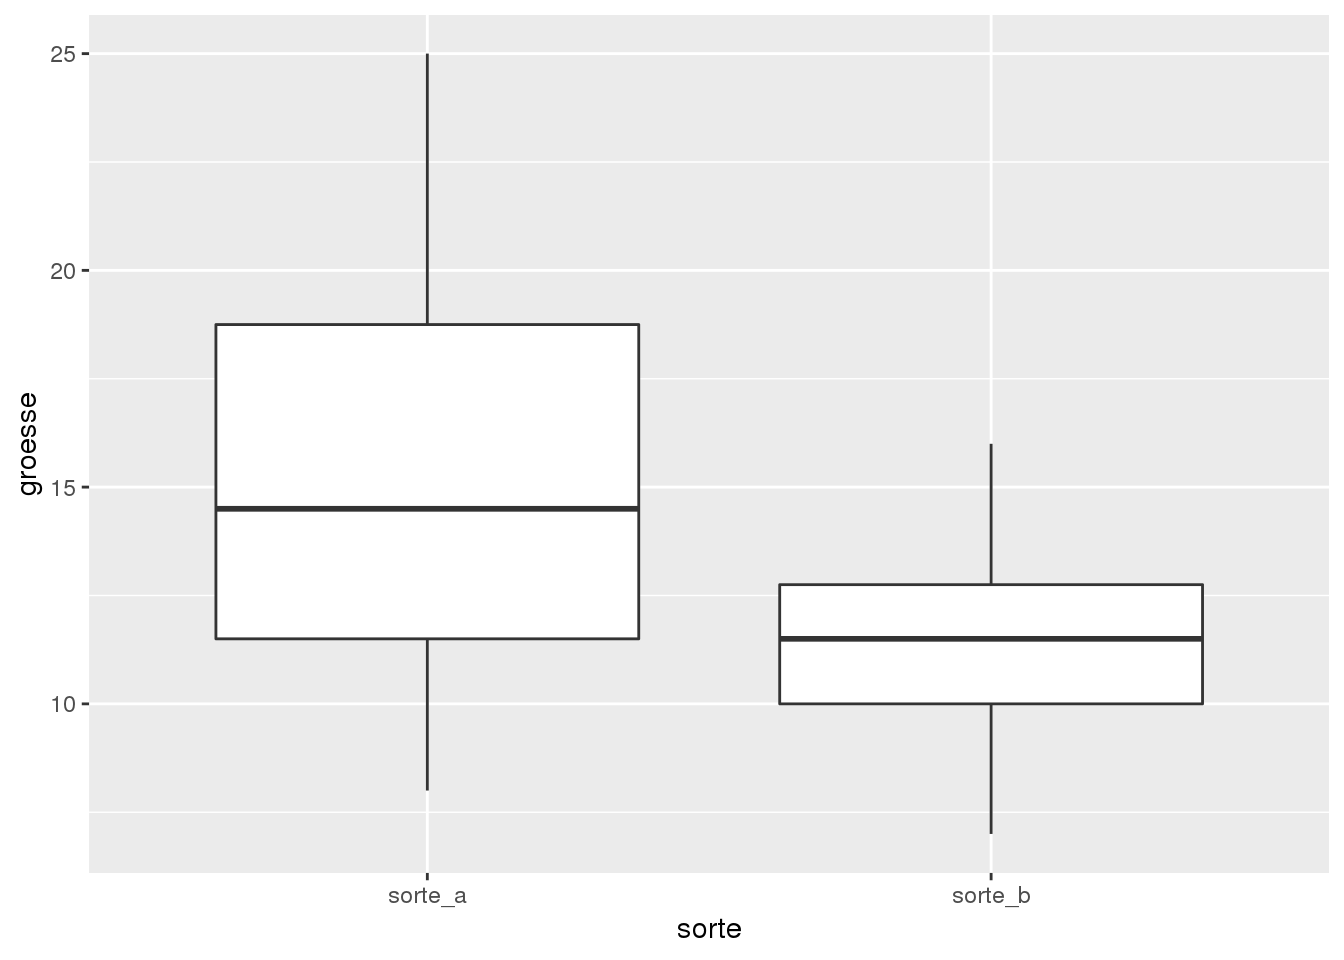
\includegraphics{_main_files/figure-latex/unnamed-chunk-27-1.pdf} 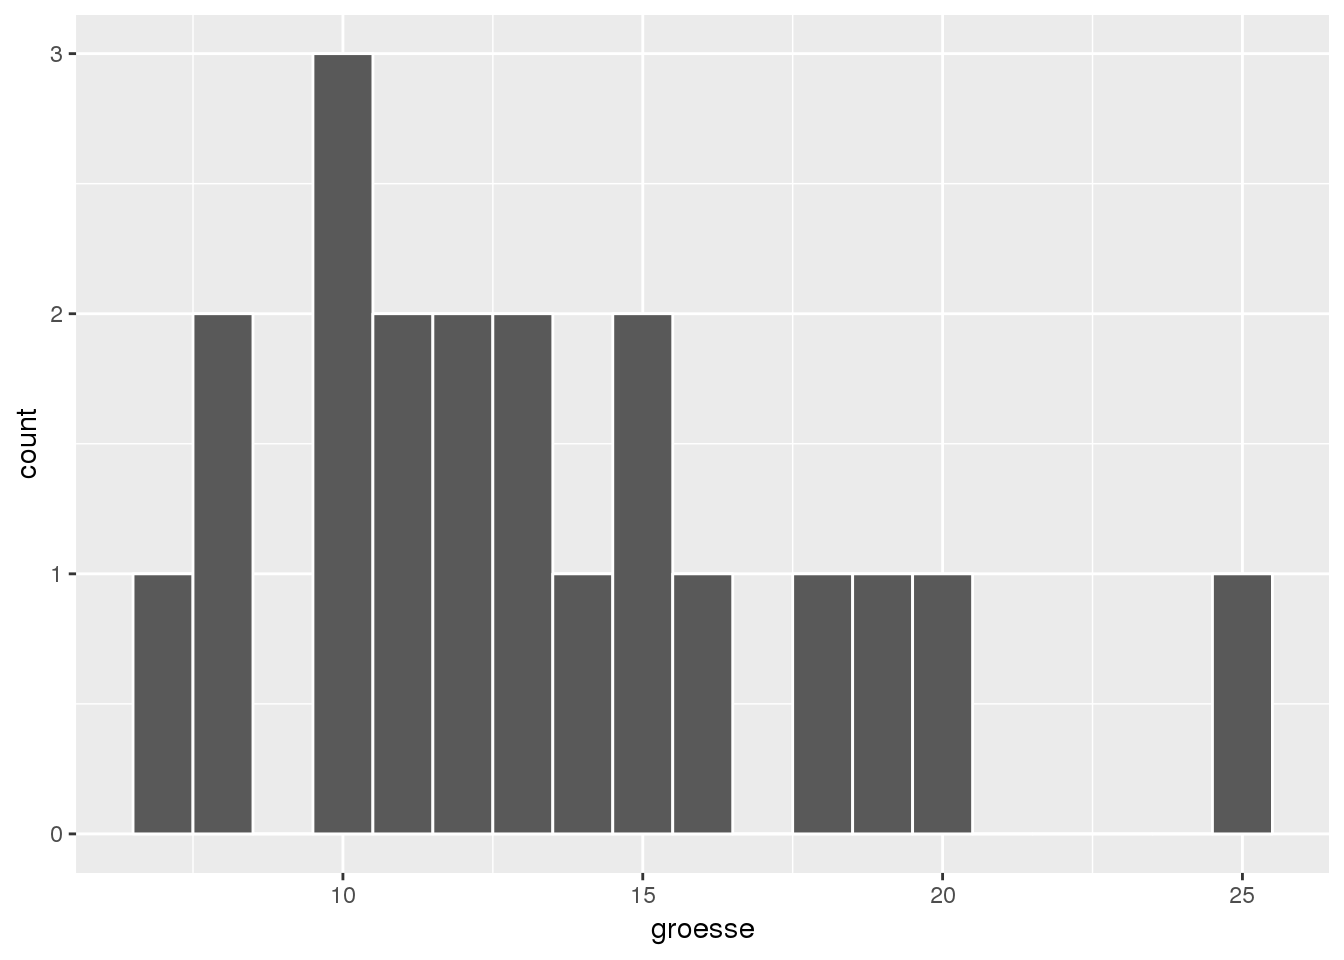
\includegraphics{_main_files/figure-latex/unnamed-chunk-27-2.pdf}

\hypertarget{aufgabe-8-fur-ambitionierte}{%
\subsection{Aufgabe 8 (für Ambitionierte)}\label{aufgabe-8-fur-ambitionierte}}

Politische Grenzen sind für die meisten natürlichen Phänomene irrelevant. Wir könnten deshalb auch eine regelmässige Kachelung (sog. Tesselierung) des Untersuchungsgebietes vornehmen. Dafür könnten wir mit \texttt{st\_make\_grid()} eine Kachelung für das gewählte Untersuchungsgebiet (\texttt{x\ =}) in einer bestimmten Grösse (\texttt{cellsize\ =}) als Quadrate (\texttt{square\ =\ TRUE}) oder sogar mit hübschen Hexagonen (\texttt{square\ =\ FALSE}) durchführen. Probier's aus!

Eine weitere, zusätzliche (und sehr anspruchsvolle) Herausforderung ist das Zeichnen und Beschriften der Kantosgrenzen. Hierzu geben wir für Wagemutige gerne Tips.

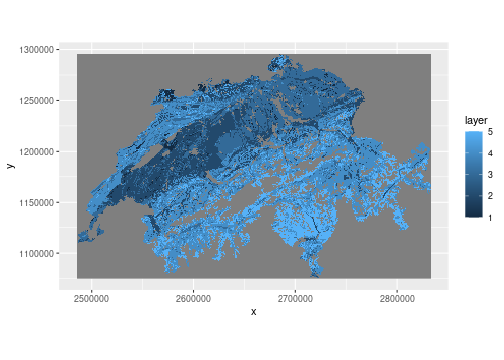
\includegraphics{_main_files/figure-latex/unnamed-chunk-28-1.pdf}


\end{document}
